\documentclass[a4paper,11pt]{report}

\usepackage[subsectionbib]{bibunits}
\usepackage{multirow}
\usepackage{longtable}
\usepackage{fullpage}
\usepackage{graphics}
\usepackage{multirow}
\usepackage[table]{xcolor}
\usepackage{graphicx}
\usepackage{pdfpages}
\usepackage{tocvsec2}
% \usepackage{natbib}
 

\newcommand{\fixedland}{{\it Fixed Landmarks}}
\newcommand{\challenge}{\paragraph{Challenge}}
\newcommand{\method}{\paragraph{Method}}
\newcommand{\approach}{\paragraph{Proposed Approach}}
\newcommand{\citep}{\cite}
\newcommand{\citet}{\cite}

\title{{\bf Modelling and Simulation of the Human Physiology:\\
Applications to the Development of Vascular Stents\\and
the Launch of the Brazilian Lung Physiome}}
\author{\LARGE{R\^omulo Teixeira de Abreu Pinho}}
\date{Science Without Frontiers Programme\\
Attraction of Young Talents\\
(60/2011 -- Third Call)\\
Project Proposal}

\begin{document}

\maketitle

\begin{abstract}
\hrule
\medskip
 As propostas deverão ser apresentadas na forma de projeto de pesquisa. Recomenda-se que este
projeto apresente as seguintes informações, de forma a permitir sua adequada análise por parte do Comitê
Julgador:
\begin{itemize}
 \item i. resumo do projeto de pesquisa proposto, incluindo objetivos e metas a serem cumpridos, com os
respectivos indicadores de desempenho;
\item ii. cronograma de execução do projeto;
\item iii. orçamento detalhado, especificando a aplicação do auxílio à pesquisa do projeto;
\item iv. grau de interesse e comprometimento de empresas ou instituições com o escopo da proposta,
quando for o caso;
\item v. descrição das atividades a serem desenvolvidas pelos demais participantes do projeto, em
especial pelo beneficiário da cota adicional de bolsa;
\item vi. disponibilidade efetiva de infra-estrutura e de apoio técnico para o desenvolvimento do projeto e;
\item vii. previsão dos ganhos e benefícios para a instituição no país com a vinda do bolsista Atração de
Jovens Talentos;
\end{itemize}

\medskip
\hrule
\end{abstract}





\tableofcontents

\chapter[Introduction]{
\hrule
\medskip\medskip\medskip
Introduction
\medskip\medskip\medskip
\hrule
}


The advance of scientific computing has fostered the development of systems to model complex biological phenoma. Possibly chief among these is the simulation of the physiology of the human body, comprising the modelling of the several multiple spatial (from 1nm for the pore size in ion channels to 1m for the size of the human body) and temporal scales (from 10-6s for the Brownian motion to 109s of our life-time), the biochemistry, the biophysics and the cellular anatomy, tissues and organs. These simulations enable both the understanding of organ functioning in normal conditions as well as the prediction of their behaviour under abnormal conditions or medical procedures. In such a way, additional information can be provided to the diagnosis and treatment of a patient and the planning of medical interventions. 

The scientific community worldwide has long been motivated by the understanding of the human physiological system. Several joint efforts and consortia have been established around the world in order to carry on research in this field. Among them, it worth mentioning the following:  

\begin{itemize}
\item Physiome Project of the International Union of Physiological Sciences \\ (http://www.physiome.org.nz/).
\item Virtual Human Project \\ (http://www.ornl.gov/sci/virtualhuman/).
\item The Digital Human Project – Federation of American Scientist \\ (http://www.fas.org/dh).
\item EuroPhysiome Project HaeMOdel – Mathematical Modeling of the Cardiovascular System \\ (http://mox.polimi.it/it/progetti/haemodel/?en=en).
\item SimBio – Simulation in Biology \\ (www.simbio.de/).
\item GEMSS – Grid for Medical Simulation Service \\ (http://www.it.neclab.eu/gemss/).
\end{itemize}

In Brazil, the most notable example of the development of systems for the modelling and analysis of human physiological systems is that of the MACC (Medicina Assistida por Computa\'c\~a Cient\'ifica) project, led by the LNCC (Laborat\'orio Nacional de Computa\'c\~a Cient\'ifica). Among the objectives of the MACC, we can emphasize


% promoted a development without precedents in the history of the human society. The popularization of the personal computer, the advent of the internet, the development of wireless communication, of the high performance distributed computing, distributed databases and data mining for knowledge discovery, monitoring techniques, scientific visualization, virtual reality, numerical simulation and computational modeling of complex systems, nowadays permeate all the human activities giving rise to huge and deep changes.
% 
% In medicine, this new reality had its roots in the beginning of the 20th Century, when it was called telemedicine (according to World Health Organization, “telemedicine is the supply of services related to healthcare when distance is a critical factor. Such services are provided by healthcare professionals, using communication and information technologies…”). However, this is currently outdated in front of the possibilities that arise with the use of the newer technologies mentioned above. For example, through the computational modeling of complex physiological systems that couple, by means of several multiple spatial scales (from 1nm for the pore size in ion channels to 1m for the size of the human body) and temporal scales (from 10-6s for the Brownian motion to 109s of our life-time), the biochemistry, the biophysics and the cellular anatomy, tissues and organs, is possible to gain insight into their functioning under normal conditions, as well as under conditions changed by pathological processes or medical procedures, giving additional information that contribute to the enhancement of diagnosis, treatment and planning of diverse medical procedures.
% 
% In this way, the scientific computation produces huge and deep changes in the medicine because it allows:
% 
% \begin{itemize}
% \item a synthesis of the image based diagnosis that, when coupled to the modeling and simulation, permits the development of new therapeutic techniques in real-time to improve medical procedures and treatments;
% \item the development of models and accurate simulators of the different systems within the human body and its inter-relation integrating anatomy, physiology, biomechanical properties, cellular biology and biochemistry for therapeutic and research applications, and also for human resources formation and training;
% \item to develop a “virtual body” for each patient in order to serve as a repository for diagnosis, pathologies and other medical information about the patient. In turn, this “virtual body” allows to increase the communication between patient and physician, furnishing a reference for exams, pathologies and changes that take place as time goes by;
% \item to make use of these models and simulators of high accuracy for surgical planning, and medical training. These simulators permit a real interaction between the user and parts of our body, represented by realistic physical and physiological properties, for educational and research purposes as well as for the development of medical applications.
% \end{itemize}
% 
% 
% Evidences of this new trend can be found in projects developed in the United States and in several countries of the European Community such as:
% 
% \begin{itemize}
% \item Physiome Project of the International Union of Physiological Sciences (http://www.physiome.org.nz/).
% \item Virtual Human Project, (http://www.ornl.gov/sci/virtualhuman/).
% \item The Digital Human Project – Federation of American Scientist (http://www.fas.org/dh).
% \item EuroPhysiome Project HaeMOdel – Mathematical Modeling of the Cardiovascular System http://mox.polimi.it/it/progetti/haemodel/?en=en).
% \item SimBio – Simulation in Biology (www.simbio.de/).
% \item GEMSS – Grid for Medical Simulation Service (http://www.it.neclab.eu/gemss/).
% \end{itemize}



The objectives of the proposed project are twofold: first we aim at developing a solution for the problem of automatic quantification of stenosis and stent choice in the treatment of vascular stenoses and aneurysms. To date, such problem has only been solved with semi-automatic methods \citep{Gremse01092011,Scherl200721,HERN-06b,Bemmel}. The goal is then to improve previous solutions with an {\em automatic} process that optimizes the {\em patient-specific} choice of stent type, length and diameter. The following sections present the main challenges involved in the project and the approaches to solve them. 




\chapter[Part I: Automatic Quantification of Vascular Stenoses and Aneurysms and the Choice of Patient-specific Stents]
{
\hrule
\medskip\medskip\medskip
Part I: Automatic Quantification of Vascular Stenoses and Aneurysms and the Choice of Patient-specific Stents
\medskip\medskip\medskip
\hrule
}

\section{Context}

Atherosclerosis is a pathology of the blood vessels that occurs when substances such as fat and cholesterol accumulate in the vessel walls, forming plaques. These plaques cause stenoses (vessel narrowing) and aneurysms (weakening and swelling of the vessel wall). Such conditions may lead to severe consequences, for example heart attacks, strokes, and the rupture of the vessel wall, all of them life threatening \citep{Gennest,Libby}. Atherosclerosis figures as one of the leading cardiovascular diseases, which remain as the major cause of death worldwide \citep{WHO}. 

Concomitantly, the use of images plays a very important role in the diagnosis, treatment, and follow up of vascular diseases. Likewise, minimally invasive interventions are becoming more available and are the preferred treatment option given the reduced surgical risk to the patient. The treatment of atherosclerosis using stents is a very good example that profits from both the use of images and minimally invasive interventions. 

A large variety of stents is available in the market. However, choosing the correct stent parameters (type, length, diameter, and deployment location) is challenging and remains a specialist-dependent and subjective task, which is mostly based on the expertise of the physician in charge. This problem attracts large attention. The multi-centre, EU-project THROMBUS\footnote{http://www.thrombus-vph.eu/}, for instance, is an attempt to understand the formation of thrombosis in cerebral aneurysms after stent implants, in order to improve stent design, choice, and deployment. An event to compare the results of existing algorithms to aid in the detection and quantification of coronary stenoses has also recently been organized\footnote{http://coronary.bigr.nl/stenoses}.

In my PhD thesis, I showed that the choice of stents for the treatment of tracheal stenosis can be automated and simplified with the use of active shape models (ASM) \citep{Cootes}. The proposed method solves the problem of automatically determining the location of the stricture, its length, and the degree of narrowing by giving an estimation of the patient's healthy trachea, that is, if stenosis were not present. From this estimation, followed by a segmentation of the narrowed trachea, determining the parameters of the stenosis and consequently of the {\em patient-specific} stent becomes a straightforward task. 

Many challenges exist when trying to use the ASMs of healthy shapes in the cardiovascular domain. First and foremost, to build the model, it is necessary to segment a large collection of healthy vascular trees and establish point-wise correspondences between them. The {\em automatic segmentation and labelling of the vascular tree} remains an open problem \citep{ORKI-08,Antiga,CARR-07,Scherl200721,Bemmel,Dikkers}. Furthermore, the {\em statistical analysis of tree-like shapes} is still in its early stages \citep{Feragen}. 

Another challenge is that when optimizing the stent choice, several parameters need to be taken into account, such as the physical properties of the vessel wall and of the stents themselves and the estimation of the blood flow after deploying the stent. In cerebral aneurysms, other constraints with respect to scale and stent properties are further taken into account \citep{larrabide:2439,Larrabide2010,bogunovic:210,zhang:1294}, although the philophy is the same as in, e.g., coronary stents. To the best of my knowledge, such parameters have only been studied in post-stent-deployment scenarios or in simulations \citep{deBeule,Florez2,Gori,Vuk,FLOR-07b,Sforza}, but have never been integrated in an {\em automatic stent choice process}, especially one that is based on ASMs. 

This project therefore aims at studying and solving the problems above and at evaluating the solutions through simulations and in the clinical domain. In order to achieve it, I would like to be part of the {\em Centre de Recherche en Acquisition et Traitement de l'Image pour la Sant\'e} (CREATIS), whose expertise in the domain of segmentation of images of the vascular system and in the use of stents in the treatment of vascular stenoses and aneurysms will be an invaluable contribution.

\subsection{Estimation of Healthy Vessels}

\challenge
When assessing vascular stenoses or aneurysms, physicians tend to pick healthy regions around the affected area in order to quantify the parameters of the deformation (extension, severity). These healthy regions in fact act as an estimation of the vessel if it were completely healthy. However, the simple selection of healthy sections may overlook shape characteristics, such as curvature, and vessels' physical properties, such as elasticity, malleability, and bending. The choice of the healthy vessel section is in fact a way to estimate the shape of the pathological region if the pathology were not present. In other words, physicians intuitively estimate how the vessel would appear if it were healthy. By doing this, they have a clearer image of the parameters of the deformation, which aids them in determining the stent dimensions and deployment location.

The {\em estimation of this healthy shape} is very subjective, much dependent on the expertise of the physician in charge. It would be desirable to devise a method in which such estimation is done automatically, taking into account the physical and geometrical properties of vessels and stents.

\approach
In \citep{Pinho:Trachea4}, a method for the estimation of healthy tracheae from CT images of patients suffering from tracheal stenosis was proposed. This method is based on the construction of an active shape model (ASM) \citep{Cootes} of 3D surfaces of healthy tracheae allied with a new model fitting algorithm, called \fixedland. When the model is registered to a CT image volume of a patient with tracheal stenosis, it is capable of matching the parts of the tracheal wall that are healthy while at the same time estimating the shape of the remaining parts as if they were healthy. The \fixedland\ algorithm is responsible for avoiding the narrowed parts of the patient's trachea, enabling the statistical model to generate a plausible healthy tracheal shape.

A natural extension of the work above is the application of the proposed 3D ASM in the cardiovascular domain. Since vessels, as well as tracheae, are objects of tubular topology, and the shape characteristics of their stenoses are roughly the same, it is intuitive to believe that the method will also be able to estimate the shape of healthy vessels from images of patients with vascular stenosis. This rule also tends to apply in the case of aneurysms, as long as there are enough healthy regions around the location of the swelling.

In this project, the method proposed for the trachea will be adapted and extended so that it can be used with narrowed and swelled vessels. In the first instance, a training set of healthy vessel sections will be built using segmentation methods available in the literature, for example \citep{Florez2}. In this way, the problem is reduced to modelling objects of tubular shape, without bifurcations, resembling the case of the trachea. Since healthy vessel sections tend to appear with good contrast in the images, their segmentation is in principle a relatively straightforward task. 

The main difficulty lies in the segmentation of the vascular tree and the corresponding surface representation to be used in the statistical model. To the best of my knowledge, very little has been done in the field of {\em statistical shape models of tree-like structures} \citep{Feragen}. In the next phase of the project, existing surface representation methods \citep{Florez, Antiga} and the corresponding branch nomenclature will be employed so as to establish correspondences between the shapes of the statistical model's training set, which is an important step in the model construction. Existing ASM fitting algorithms will be extended to cope with the possible new difficulties when registering the model to deformed vessels. New fitting algorithms will also be developed to account for bifurcations. At this stage, only geometrical properties of the vessels will be taken into account. The inclusion of physical properties of vessels and stents in the model are discussed later in the text. 

\subsection{Segmentation of the Vascular Tree}

The segmentation of the vascular tree has been a topic of study for quite some time, but the automatic segmentation remains an open problem \citep{ORKI-08}. In the context of this project, the segmentation task is subdivided into two objectives: 1) the segmentation of healthy vascular trees; 2) segmentation of vessels with stenosis. Each is detailed in the following sections.

\subsubsection{Healthy Vascular Trees}

\challenge

ASMs depend on the selection of a large set of training shapes, whose geometrical variation is encoded in the model. The segmentation of the healthy vascular tree is thus an important step in the construction of the model. 

\approach

This segmentation problem has much in common with the segmentation of the airway tree. Despite also being an open problem, automatic segmentation algorithms for the airways exist and were even been evaluated in a recent segmentation challenge\footnote{http://image.diku.dk/exact/}. One of these algorithms \citep{Pinho:Airways2} implements an iterative region growing with adaptive, cylindrical ROIs that employs anatomical information in the detection and elimination of leaks, a common problem in region growing. The method also includes an initialization step to automatically detect the starting point of the trachea, which is given as a seed point to the region growing algorithm. 

%\begin{figure}%
%\centering
%\includegraphics[width=0.5\columnwidth]{research_interests_airways.jpg}%
%\caption{Segmentation of the airway tree as proposed in \citep{Pinho:Airways2}.}%
%\label{fig:airways}%
%\end{figure}

The intention is to adapt and extend the referred method to the segmentation of healthy vessels and to compare it with other (semi-)automatic methods \citep{Zhou20121,CARR-07,FLOR-07b,Florez2,Scherl200721,Antiga,Bemmel}. In order to detect a seed point for the region growing algorithm, tube enhancement filters \citep{ORLO-09} may help in at least isolating the tubular structures in the image, from where the detection process may be triggered. 

\subsubsection{Pathological Vessels}
\label{sec:narrowedarteries}

\challenge
Similarly to the case of tracheal stenoses, segmenting the narrowed vessels is an important step in the automatic calculation of the parameters of the vessel stricture. Previous experience with the segmentation of the trachea, however, has demonstrated that the segmentation of narrowed tube-like structures in medical images may be difficult \citep{Triglia,Pinho:Trachea7}. Region growing, for example, tends to fail to recover the correct tube wall if the narrowing is too severe and the lumen is not completely visible in the image. 

\approach

In \citep{Pinho:Trachea4}, an estimation of the patient's healthy trachea was used as initialization of a deformable model to segment the narrowed tube. The proposed deformable model, based on the snake model proposed by \citep{Kass}, was able to correctly segment the tracheal wall even in the more difficult cases. 

I will thus experiment with the referred deformable model in order to automatically segment narrowed vessels. The idea will still be to initialize the model with the estimation of the healthy vessel obtained with the ASM. This method should give better results then other solutions in the literature \citep{CARR-07,Florez2,Antiga,Bemmel}, but an in-depth comparison with those algorithms will be necessary.

\subsection{Stent Choice}

Physicians intuitively estimate the healthy shape of the narrowed vessel when quantifying the stenosis or the aneurysm. The solutions proposed above should be able to mimic the physician's work in a methodological and mathematical manner. After the estimation of the healthy vessel shape, we are ready to automatically detect the exact location of the stenosis and to quantify it. For this, it is necessary to track changes in the cross-sectional area of the narrowed tube relative to the estimated healthy tube \citep{Pinho:Trachea4} or relative to selected healthy vessel sections \citep{Florez2,Bemmel}.

Once the stenosis or aneurysm has been detected and quantified, the parameters of the stent are trivially obtained. At this point, the whole chain of the proposed project will be finished. However, the effectiveness of the predicted stent can only be verified after it has been deployed in the patient's vessel. If the stent is inadequate, it may migrate to another location or strain the vessel wall. 

For this reason, I will add to the stent choice process several parameters derived from the physical properties of the vessel and of the stent itself. In addition, every predicted stent will be used in a blood flow simulation step such that its effectiveness can be further verified. From the simulations, other parameters will be extracted and added to the decision process. In this way, the proposed method will be turned into an optimization process on several variables. Some of them will impact the estimation of the vessel's healthy shape, some will impact the stent choice.

\subsubsection{Extending the Statistical Shape Model}

\challenge
The registration of the ASM of healthy vessels to an image of a patient with atherosclerosis is an iterative, edge-based search. At each iteration, the new locations of the landmarks that describe the surface of the vessel are determined and a least squares minimization process makes the shape generated by the ASM fit to the new point locations. Since the model is constrained by the (healthy) shape information contained in it, the resulting surface will resemble a healthy vessel.

A ``healthy vessel'' in this context means that only the geometrical variation about the vessels is captured by the statistical model. Still, vessels have physical properties such as elasticity, malleability, and bending, that are not explicitly encoded in the model. At the best, the geometric information may implicitly contain some aspects of the referred properties. 

\approach
I will then collect the physical properties of vessels available in the literature \citep{ZAHN-11d,BOUS-09c,BOUS-08c,SULA-08a,Oubel,zhang:1294,Balocco} in order to add such information to the 3D ASM. As a result, when registering the model to the patient's image these properties will further constrain the deformation, which should help in obtaining a better estimation of the healthy vessel shape. 

In the same way, I will further extend the ASM with the physical properties of the stents. Since the ultimate objective of the project is the automatic prediction of patient-specific stent parameters, it is reasonable that their physical properties be an extra parameter in the construction of the model. Consequently, when registering the model to the patient's image, not only will the properties of the vessel play a role, but we will at the same time influence the estimation of the healthy vessel with the properties of the stent. The novelty here will be the combination of geometric (shape) and non-geometric information into a multi-dimensional ASM. 

\subsubsection{Physically-based Segmentation of Pathological vessels}

\challenge
In the same way that the statistical shape model can be extended, so can be the segmentation of narrowed and swelled vessels. Originally, the snake model proposed in \citep{Kass} depends on internal and external energies to deform the surface towards the desired image feature. The internal energies take only elasticity and bending into account. 

\approach
I will add extra energy terms taking into account vessels' physical properties \citep{BOUS-09c,ZAHN-11d}, in order to restrict (or improve) the surface deformations, so that the model can better adapt to the vessels' boundaries. Such physical properties must also take into account those of narrowed and swelled regions, since the main object of this segmentation step is to correctly segment them.

\subsubsection{Simulations}

\challenge
As stated previously, when the estimated healthy vessel shape and the segmented narrowed vessel are obtained, the automatic detection and quantification of the stenosis or aneurysm tends to be trivial. The stent to be chosen, however, is the one that will optimize the blood flow after deployment. 

Blood flow simulations already play an important role in stent design and placement planning \citep{deBeule,ATTI-08}. They are also extensively used for flow assessment after stent deployment \citep{Vuk,Gori}. However, to the best of my knowledge, such simulations have not yet been integrated in a method or algorithm for the stent choice process. 

\approach
In \citep{Florez,deBeule}, methods were proposed for stent deployment simulations using deformable models and numerical methods. With these methods, it is possible to (visually) verify whether the predicted stent properly expands the narrowed region of the vessel or whether it correctly bypasses the swelled region. 

The idea is then to methodologically quantify these parameters, by using the stents' and vessels' physical properties, and to have measures for, e.g., vessel wall straining, stenosis/aneurysm coverage, stent deformation, etc \citep{BOUS-09c,BOUS-08c,SULA-08a}. These parameters can be further added to the ASM so as to improve the healthy shape estimation. Consequently, the ASM registration will tend to yield a shape with the best characteristics in terms of the stent vs. wall interaction as well.

To achieve the integration of blood flow simulation with the stent choice, the plan is to define a function of the blood flow subject to the stent parameters (physical properties, deployment location, length, and diameter). This function will then be maximized, such that the chosen stent is the optimal one for a certain patient. This optimization process will thus influence the entire workflow, from the estimation of the healthy vessel shape, passing through the segmentation of the narrowed/swelled vessel, to the detection and quantification of the stenosis/aneurysm, and the final prediction of the stent parameters. In fact, we imagine an algorithm that implements the workflow depicted in Figure \ref{fig:workflow}. 

\begin{figure}%
\centering
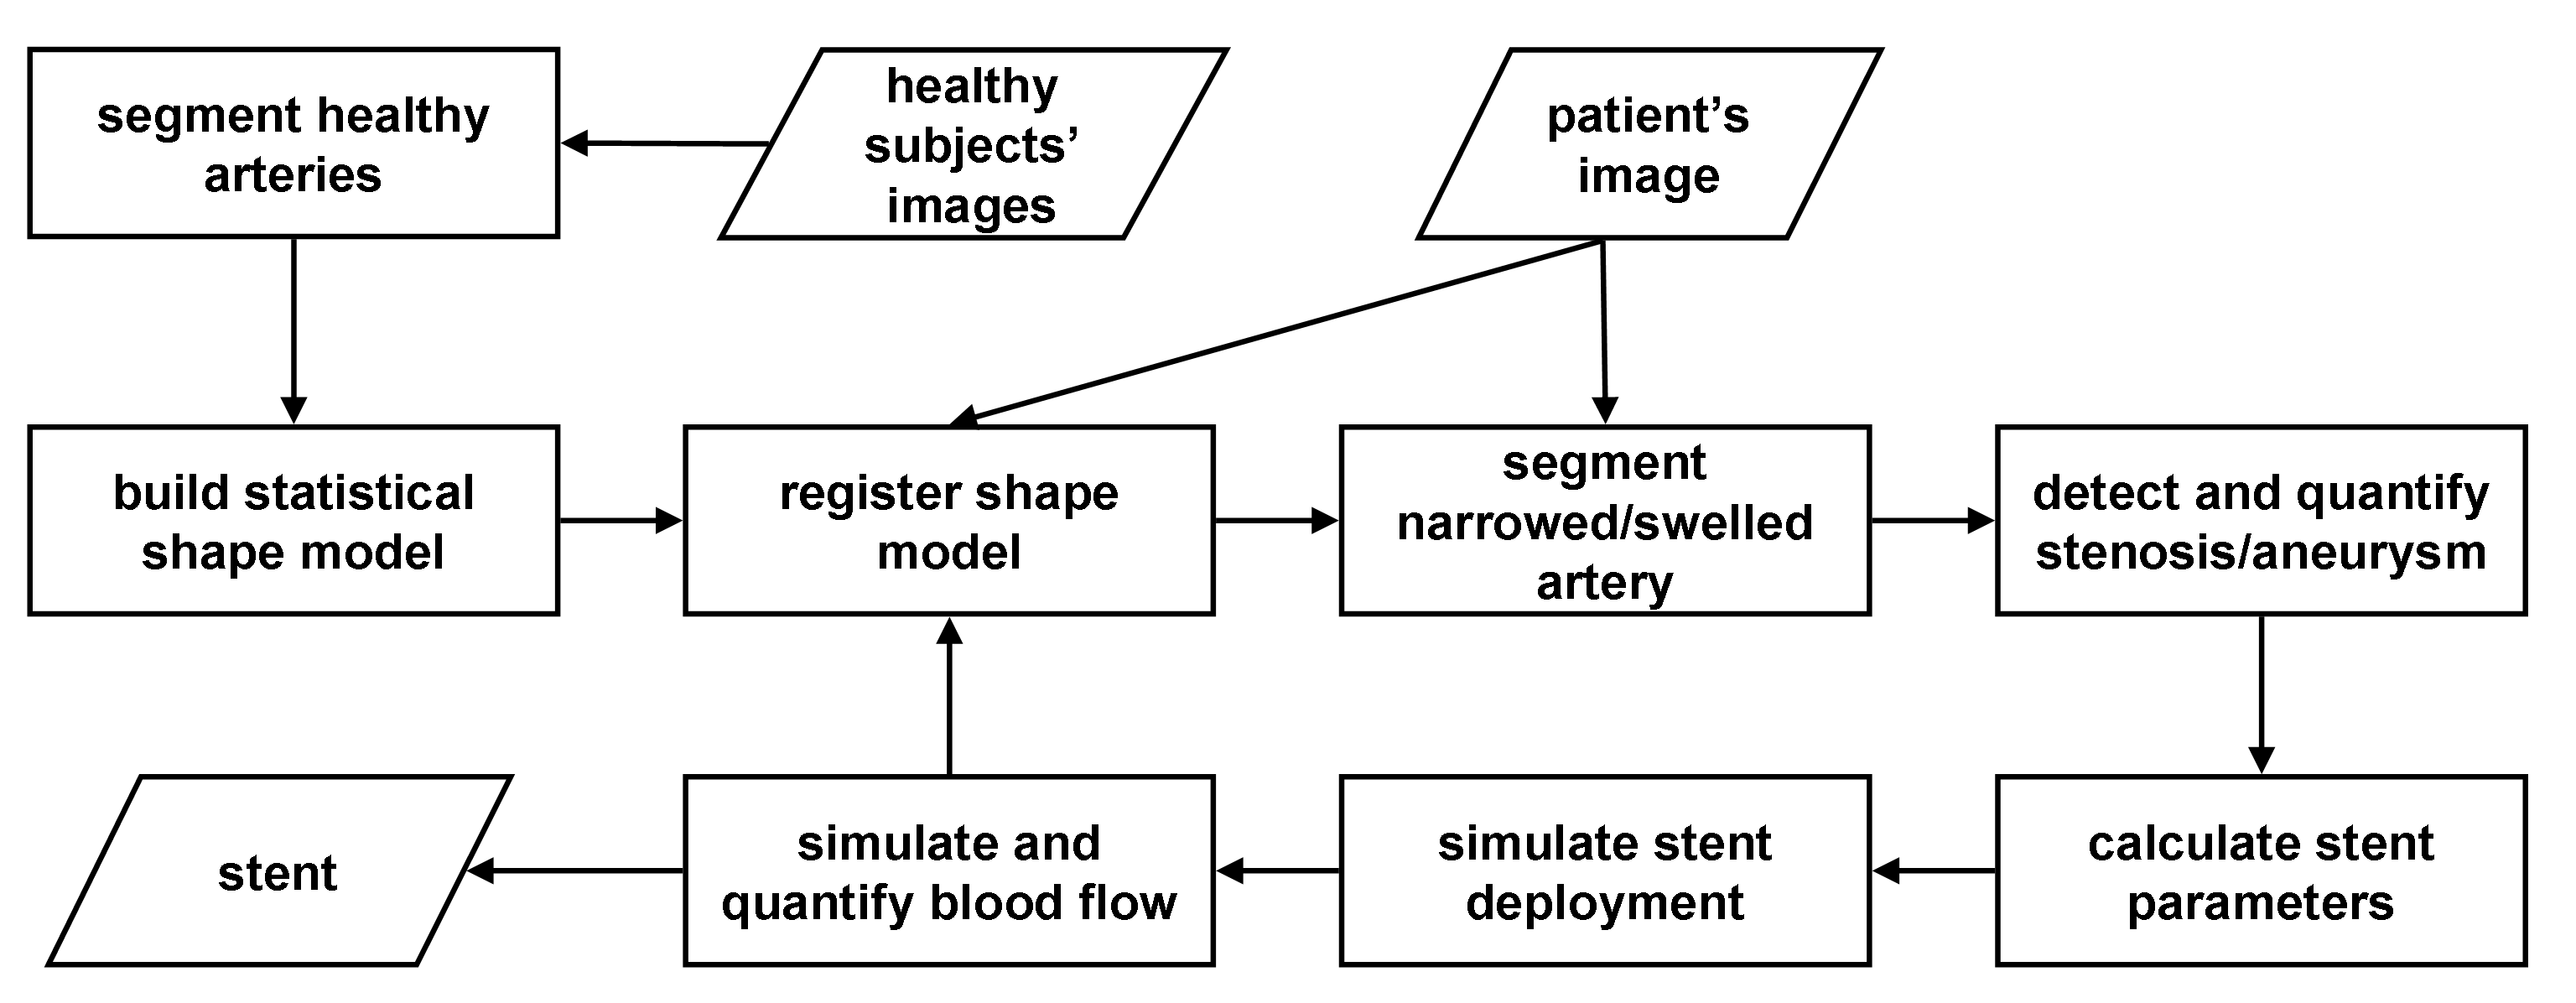
\includegraphics[width=0.8\columnwidth]{workflow.png}%
\caption{Workflow of the complete automatic stent prediction process.}%
\label{fig:workflow}%
\end{figure}

\subsection{GPU Acceleration}

\challenge
In order to achieve the expected results with the proposed methods, a lot of computational power may be necessary. The blood simulations, for instance, are very computation intensive (e.g., 48 hours running on a 200-CPU cluster \citep{deBeule}). The proposed optimization process, as well, is a classic case study for the use of clusters and grids, given the number of potential variables in the problem. I envision the use of such architectures, but bringing them to the clinic is impractical and expensive. A more viable, yet powerful, solution is thus necessary.

The FASTRA\footnote{http://fastra.ua.ac.be/en/index.html} technology is a successful attempt of building a desktop supercomputer using multiple GPUs. At the cost of a couple of high-end desktop computers, this technology yields computing power comparable to more than 256 CPUs working together, with proper GPU programming.

In GPU programming, however, the size of the data to process may be larger than the available GPU memory. In this case, we need to be selective about which parts of the data should be transferred to the GPU memory at each time. In this project, it is possible that the areas of interest in the image, that is, those with the vessels under study, occupy a small part of the image. Careful identification of this part of the image could minimize data transfers between RAM and GPU. 

\approach
In \citep{Pinho:Cache1}, a similar problem was dealt with, but in a different scale. Since image processing pipelines may require several simultaneous copies of the image buffer, current available RAMs may not be large enough. An out-of-core solution for image processing based on sliding window cache and pre-fetching techniques was then proposed. In other words, only the parts of the image that are necessary in a given moment reside in main memory. The other parts remain in disk. Using a-priori knowledge about the image traversal pattern of image processing algorithms, it is possible to predict which regions of the image will be needed in the future. These images can be asynchronously fetched from disk and stored in a cache before being requested by the algorithm. If the I/O operation is fast enough, it is very likely that the algorithm will not have to wait for the request complete. 

The method above can similarly be applied in the selection of what data to bring to the GPU. I will then analyse the image traversal patterns of the algorithms developed in this project and develop new cache and pre-fetching strategies for the GPU vs. RAM architecture. In this way, the stent choice optimization can potentially be made in the clinic without the need of the cluster structure.




\chapter[Part II: The PulMoLab]
{
\hrule
\medskip\medskip\medskip
Part II: The PulmoLab
\medskip\medskip\medskip
\hrule
}
\label{chap:pulmolab}

\section[Context]{Context}

The need for a quantitative understanding of in vivo lung function leads to the need for reliable model representation of the in vivo lung structure. The lung primarily comprises parenchymal (gas exchange) tissue, airways, arteries, and veins. The treelike structures of the airways and blood vessels are intimately bound to—and suspended within—the parenchyma (alveolar tissue). Function in the lung is strongly influenced by the spatial positioning of the airways and vessels \citep{TawhaiM2011,Tawhai2010}, calling for a patient-specific approach in simulating and analysing lung structure and function. 

With advances in modern medical imaging and the steady and rapid increase in computing power, it is now possible to derive models that replicate the many geometric features of individual lungs, and to simulate function within these geometric models, taking into account their different spatial and time scales \citep{Tawhai2010,Tawhai2000,Tawhai08,Burrowes2005}.

A number of international projects have put together groups interested in the modelling and simulation of lung function, among them the Human Lung Atlas \citep{Hoffman2004,Li2003}, the Lung Physiome \citep{TawhaiM2011}, and the AIRPROM-VPHNoE\footnote{http://cordis.europa.eu/projects/rcn/97980\_en.html}. In Brazil, to the best of my knowledge, such an effort has not yet been started. However, patient-specific modelling and simulation of the human cardiovascular system has been a topic of interest of the HeMoLab group of the LNCC since 2005, and also part of the nation-wide project MACC. 

Computational modelling and simulation of the cardiovascular system is fundamentally similar to modelling and simulation the physiology of the lungs and the gas exchange process. The main interest of this part of the proposed project is thus to extend the work developed by the HeMoLab group in the context of the MACC project \citep{Blanco2012,Blanco2010,Blanco2009a,Blanco2007,Golbert2012,Malossi2011,Urquiza2006}, adding to it the modelling of the gas exchange process. The primary objective is to investigate the existing literature on the subject, find the common points with the work developed in the HeMoLab, and carry out the integration between the existing models of vascular system and the new models of gas exchange. Some challenges in this process are rather clear, which are show below along with the approaches to solve them. 

\section{Segmentation of the Airway Tree}

\challenge

It has been shown that CFD simulations of airflow are largely improved when patient-specific image based models of the airways are employed \citep{Tawhai2010,Vial2005}. In effect, the segmentation of the airway tree has been a topic of study for quite some time, but the automatic segmentation remains an open problem. Achieving correct manual (or semi-automatic) segmentation can be painstaking, non-reproducible, and prone to error. Yet, state-of-art, fully automatic algorithms still fall short of achieving the same results obtained with manual interventions \citep{Lo}. The complexity lies in the little image resolution at the lower levels of the airway tree. Noise and other artefacts such as partial volume effect make the automatic identification of smaller branches even more difficult.

\approach

One algorithm for the automatic segmentation of airway trees \citep{Pinho:Airways2} implements an iterative region growing with adaptive, cylindrical ROIs that employs anatomical information in the detection and elimination of leaks, a common problem in region growing. The method also includes an initialization step to automatically detect the starting point of the trachea, which is given as a seed point to the region growing algorithm. 

The intention is to further extend the referred method and try to incorporate new ideas from the litterature \citep{Lo} in order to increase the branch detection count and to reduce the number of segmentation leaks and false positves. For example, tube enhancement filters \citep{ORLO-09} may help in at least isolating the tubular structures in the image, from where the detection process may be triggered. Branch generation algorithms \citep{Tawhai2000} will also be investigated.

\section{Segmentation of the Pulmonary Vascular Tree}

\challenge

The vessels that compose the pulmanary vascular tree have a many-to-one relationship with the airway bronchi. Namely, each bronchial airway is related to one arterial vessel, but there are more arteries than branches of the airways. The same applies to the venous system. These extra vessels, referred to as "supernumerary", together with the other vessels are responsible for transporting blood to the gas exchange surface, within the lung parenchyma. Correct modelling of the vessel tree is thus an important step in trying to perform gas exchange simulations. Therefore, it is necessary to correctly segment the vascular tree in order to obtain valid patient-specif geometric models to be used in the CFD simulations. 

\approach

In theroy, the algorithms proposed for the segmentation of the airways can be employed in the segmentation of pulmonary vascular tree, for the two trees have, overall, the same strucutre \citep{TawhaiM2011}. Therefore, we will investigate the use of the algorithms described in \citep{Lo}, for the airways, and also those proposed exclusively for the segmentation of the vascular tree, such as \citep{Dongen,Ebrahimdoost,Gutierrez,Linguraru,Shikata,Wala}.


\section{Patient-specific Airflow and Gas Exchange Simulations}

\challenge

An appropriate multiscale model will capture the important features of function at each spatial or temporal scale while maintaining as much computational simplicity as possible. Physical forces acting on the surface of the intact lung are transmitted to the level of the gas exchange tissue (where they hold open the small airways and blood vessels) and on down to the level of cells and molecules where stress modulates local function. Conversely, chemical reactions at the molecular level eventually trigger changes in the shape of the lungs and of the airways to, for example, increase or decrease breathing speed.

Correct, patient-specific modelling and simulation of the gas exchange process depends ....

On the one hand, this is probably the most challenging part of the PulMoLab proposal. On the other hand, it is also the one that tends to benefit the most from the expertise of the MACC/HeMoLab/LNCC in the modelling and simulations of the human vascular system. 

\approach

The main objective in this part of the project is to study the work about modelling and simulations of gas exchange available in the recent literature, for example \citep{TawhaiM2011,Tawhai2010,Tawhai08,Burrowes2005,Lin2009,Werner2009,DeBacker2008,DeBacker2010,Gemci2007}. At the same time, it will be necessary to get fully acquainted with the work developed at the HeMoLab group about the cardiovascular system, most notably \citep{Blanco2007,Blanco2009a,Blanco2010,Blanco2012,Urquiza2006}. The next step will be to find opportunities for innovation so as to carry out the proposed extension of the work developed at the MeMoLab.

\section{Correlations Between Pulmonary Structure and Function}

\challenge

As stated before, one the most significant benefits of airflow and gas exchange simulations is to establish correlations between lung structure and function. In other words, the aim to answer questions such as how the shape of the airways influences turbulence of the airflow or particle deposition, or how the geometry of the lungs and its deformations upon breathing affect the overall gas exchange process in the normal patient or in the presence of diseases. 

\approach

Since the aim is to find correlations in which shape variations are involved, the idea is to employ the aforementioned Active Shape Models (ASMs) \citep{Cootes} for this task. To the best of my knowledge, ASMs have never been used to correlate lung shape and function. Furthermore, the reader is reminded that research on the {\em statistical analysis of tree-like shapes}, e.g., the airway tree, is still in its early stages \citep{Feragen2011,Feragen2012}, so there may be many opportunities for innovation is this case. This approach will benefit from the results obtained with the estimation of healthy arteries, described in Section \ref{sec:healthyvessels}, and vice-versa.



\chapter[Integration in the Laboratory and Collaborations]
{
\hrule
\medskip\medskip\medskip
Integration in the Laboratory and Collaborations
\medskip\medskip\medskip
\hrule
}
\label{chap:integration}

\section{Laboratory}

My intention of joining the HeMoLab project of the LNCC is on the one hand to benefit from their expertise in the several areas correlated to this project proposal. In particular, as mentioned before, HeMoLab/LNCC is the leading research group of the MACC project, among the objectives of which is the development of models of blood circulation \citep{}. On the other hand, it will be my role to contribute to group's expertise by 1) bringing to the lab my own experience with the automatic assessment and patient-specific stenting of tracheal stenosis and applying it to the cardiovascular domain and 2) building upon the group's existing work on the cardiovascular system to develop the proposed PulMoLab project.

HeMoLab/LNCC also have at their disposal two internal computer clusters for large scale computations. Their expertise in the parallel computing domain and the processing of massive image data have been demonstrated through their participation in many nationwide projects, such as the MACC itself. This cluster is part of a larger grid structure comprising several research instutions across the country, the SINAPAD\footnote{https://www.lncc.br/sinapad}, of which the LNCC is the coordinating instution. Such expertise and tools will be invaluable for the simulation parts of the proposed project. 

Most importantly, HeMoLab/LNCC also profit from a very multidisciplinary nature and strong links with the clinical practice, most notably that of the {\it Instituto do Coração} (Incor), in S\~ao Paulo. This will potentially give me the opportunity to evaluate the results of the proposed project with real patient data and to have immediate feedback from physicians. 

\section{Collaborations}

During my PhD in Belgium, I established a very good relationship with Prof. Dr. Jan Sijbers, my thesis supervisor, in the VisionLab group of the University of Antwerp. The group has extensive experience with medical image segmentation problems and modelling of cylindrical objects, which could be interesting in the context of this project. In addition, this is the group where the FASTRA technology for GPU acceleration was developed, and they are always interested in new applications for it. I would like to bring the VisionLab and the HeMoLab/LNCC together during the course of the proposed project, so that they can benefit from each other's work.

My stay in Belgium also allowed me to get acquainted with the work of the Stent Research Unit of the University of Ghent. Since their work is focussed on the design of stents using numerical simulations, on which much of this project may be based, it is a potential collaboration opportunity. 

We also envision collaborations with the academic and industrial partners of the European Project THROMBUS, whose aim is to evaluate the efficacy of the use of stents in neurological aneurysms, and researchers involved with the state of the art in gas exchange modelling and simulations. Likewise, we would to be in close contact with the research groups involved in the Lung Physiome project, possibly the leading researchers in the field. All these groups combine expertise in different areas and will certainly be a good source of information for this project.

\chapter[Schedule and Use of Funding]
{
\hrule
\medskip\medskip\medskip
Schedule and Use of Funding
\medskip\medskip\medskip
\hrule
}
\label{chap:schedule}
\section{Tentative Schedules}

Due to relocation issues, I intend to start working on this project in March 2013, wich is the limit start date of this call. Having this plan in mind, below are two tables with tentative schedules for the each part of this project proposal.

\paragraph{Part I}
The objective in the short term, roughly the first 6 months, is to try to directly apply the ASM used for the trachea to cases of vascular stenosis and aneurysms. There are reasons to believe that this step tends to be rather straightforward, requiring only few modifications to the original method, if any. The possibly biggest challenge would be the segmentation and surface modelling of the vessels, which, in the first instance, could be simplified (e.g., not taking bifurcations into account) and accomplished with existing techniques so as to yield acceptable results in a short period of time. 

The following step, to be carried out during the next 18 months, will be the extension of the ASM with anatomical information about the vascular tree. Bifurcations will also be taken into account. 

Finally, the remaining 12 months will be dedicated to the stent choice and simulation parts. The starting point of this step will be the stent choice with a generic stent and vessel model. In other words, stents' and vessels' physical properties will not be taken into account. In this way, we will be able to at least evaluate if the generic stents computed with the ASM are adequate. Later, blood flow and stent deployment simulation results will be used to improve the statistical model and, ultimately, the automatic stent choice.  

\begin{table}[h]\centering
\begin{tabular}{c|c|c|c|c|c|c|}
\cline{2-7}
 & \multicolumn{2}{|c|}{Y1} & \multicolumn{2}{|c|}{Y2} & \multicolumn{2}{|c|}{Y3} \\ \cline{2-7}
 & S1 & S2 & S3 & S4 & S5 & S6 \\ \hline
\multicolumn{1}{|c|}{Apply existing model} & \cellcolor{green} & & & & & \\ \hline
\multicolumn{1}{|c|}{Segmentation and modelling} & & \cellcolor{green} & \cellcolor{green} & \cellcolor{green} & & \\ \hline
\multicolumn{1}{|c|}{Stent choice and simulations} & & & & & \cellcolor{green} & \cellcolor{green} \\ \hline
\end{tabular}
\caption{Part I -- Tentative schedule for 3 years, subdivided into semesters.}
\label{tab:schedule1}
\end{table}

\paragraph{Part II}

\begin{table}[h]\centering
\begin{tabular}{c|c|c|c|c|c|c|}
\cline{2-7}
 & \multicolumn{2}{|c|}{Y1} & \multicolumn{2}{|c|}{Y2} & \multicolumn{2}{|c|}{Y3} \\ \cline{2-7}
 & S1 & S2 & S3 & S4 & S5 & S6 \\ \hline
\multicolumn{1}{|c|}{Apply existing model} & \cellcolor{green} & & & & & \\ \hline
\multicolumn{1}{|c|}{Segmentation and modelling} & & \cellcolor{green} & \cellcolor{green} & \cellcolor{green} & & \\ \hline
\multicolumn{1}{|c|}{Stent choice and simulations} & & & & & \cellcolor{green} & \cellcolor{green} \\ \hline
\end{tabular}
\caption{Part II -- Tentative schedule for 3 years, subdivided into semesters.}
\label{tab:schedule2}
\end{table}


\section{Use of Funding}

I will be the coordinator and main researcher in proposed project and therefore the direct benefiter of offered grant. However, I acknowledge that the project is rather ambitious and I that will not be able to work on it alone. Some of the challenges described above may solved in the context of Master or even PhD theses, funding for which may be available from the usual Brazilian funding bodies. Yet, I am convinced that it will be necessary to hire an extra research engineer for the entire duration of the project (three years), who will mostly take care of implementing the algorithms devised to solve the challenges and those from the literature that may be useful. Consequently, part of the extra research funding (R\$ 20.000,00/year) will be emplyed in the purchase equipment for myself and for the hired engineer. Occasionally, part of this funding may also be used for trips to collect data, in case they cannot be transfered electronically.


\bibliographystyle{apalike}
\bibliography{mybib,trachea,stents,artery,cfd}

\appendix
\settocdepth{chapter}
\chapter[Curriculum Vit\ae]{
\hrule
\medskip\medskip\medskip
Curriculum Vit\ae
\medskip\medskip\medskip
\hrule
}

\section{Contact Information}

40, Rue Colin\\
Villeurbanne, 69100, France.\\
Mobile Number: +33-(0)-638305900\\
e-mail: romulo.pinho@lyon.unicancer.fr\\
URL: www.creatis.insa-lyon.fr/rio/RomuloPinho

\section{Biographical Data}

Birth date: March, 3rd, 1977\\
Place of Birth: Petr\'opolis, RJ, Brazil\\
Citizenship: Brazilian\\
Marital status: Married

\section{Current Position}

\begin{longtable}{p{0.25\textwidth} p{0.6\textwidth}}
January, 2011 \newline present & Post-doc Research Engineer \newline
Centre L\'eon B\'erard, Lyon, France \newline
Design, implementation, and deployment of a medical imaging system for image guided
radiation therapy against lung cancer. The aim is to carry out a clinical trial for the use of new
image registration techniques and their influence on radiation therapy against moving tumours. 
Multi-platform development using C++, CMake, ITK, VTK, QT, Python, and shell scripts.\\
\\
\end{longtable}


\section{Education}

\begin{longtable}{l p{0.6\columnwidth}}
November, 2010 & Ph.D. in Physics. \newline 
Universiteit Antwerpen, Antwerp, Belgium \newline 
Specialization: Medical Image Processing \newline 
Thesis: A Decision Support System for the Assessment and Stenting of Tracheal Stenosis. \\
\\
May, 2001 & M.Sc. in Software Engineering. \newline 
Universidade Federal do Rio de Janeiro, Rio de Janeiro, Brazil \newline 
Specialization: Computer Graphics \newline 
Thesis: Three Dimensional Reconstruction of Head Models from Magnetic Resonance Images. \\
\\
September, 1998 & B.Sc.  in Computer Science \newline 
Universidade Federal Fluminense, Niter\'oi, Brazil \newline 
Specialization: Computer Science.\\
\end{longtable}


\section{Honours, Awards and Certificates}

\begin{tabular}{p{0.25\columnwidth} p{0.6\columnwidth}}
Las Vegas, April, 2005 & ScrumMaster Certificate.
\end{tabular}

\section{Languages}

\begin{tabular}{l p{0.6\columnwidth}}
Portuguese & native\\
English & fluent (non-native)\\
French & intermediate level\\
Dutch & basic level\\
\end{tabular}

%\renewcommand{\refname}{Contributions}
%\begin{bibunit}[unsrt]
%\bf{Book Chapters} \\
%\nocite{Pinho:Cache1}
%\nocite{Pinho:Cache2}
%\bf{Journals} \\
%\nocite{Pinho:Airways1}
%\nocite{Pinho:Airways2}
%\bf{Conference Papers (full paper)} \\
%\nocite{Pinho:Trachea1}
%\nocite{Pinho:Trachea2}
%\nocite{Pinho:Trachea3}
%\nocite{Pinho:Trachea4}
%\nocite{Pinho:Trachea5}
%\nocite{Pinho:Trachea6}
%\nocite{Pinho:Trachea7}
%\putbib[mybib]
%\end{bibunit}

%\bibliographyunit[\section]
\section{Scientific Publications}

\renewcommand{\refname}{Journal papers}
\begin{bibunit}[unsrt]
\nocite{Pinho:Airways3}
\nocite{Pinho:Trachea7}
\nocite{Pinho:Trachea4}
%\nocite{Pinho:Cache2}
\putbib[mybib]
\end{bibunit}

\renewcommand{\refname}{Book chapters}
\begin{bibunit}[unsrt]
\nocite{Pinho:Trachea5}
\putbib[mybib]
\end{bibunit}

\renewcommand{\refname}{Conference proceedings (full paper)}
\begin{bibunit}[unsrt]
\nocite{SARRUT-12}
\nocite{DELM-11}
\nocite{PINH-11}
\nocite{RIT-11b}
\nocite{Pinho:Trachea6}
\nocite{Pinho:Airways2}
\nocite{Pinho:Trachea3}
\nocite{Pinho:Trachea2}
\nocite{Pinho:Cache1}
\nocite{Pinho:Trachea1}
\nocite{Pinho:Airways1}
\putbib[mybib]
\end{bibunit}

\renewcommand{\refname}{Conference proceedings (abstract)}
\begin{bibunit}[unsrt]
\nocite{Bernat:Clavicle}
\nocite{Huysmans:Clavicle}
\nocite{Pinho:Trachea8}
\putbib[mybib]
\end{bibunit}


\section{Academic Experience}

\subsection{Teaching}
\begin{tabular}{p{0.25\columnwidth} p{0.6\columnwidth}}
September, 2011 \newline June, 2012 & Teacher assistant \newline
Subject: Operating Systems \newline
(in French, 16h, practice sessions) \newline
Institution: INSA-Lyon\\
\\
September, 2011 \newline June, 2012 & Teacher assistant \newline
Subject: Object Oriented Programming \newline
(in English, 45h, theory and practice sessions) \newline
Institution: INSA-Lyon\\
\\
\end{tabular}

\subsection{Supervision of Theses}
\begin{tabular}{p{0.25\columnwidth} p{0.6\columnwidth}}
January, 2009 \newline June, 2009 & B.Sc. Thesis of Stijn Peeters (co-supervision) \newline
Title: Automatic segmentation of the airways: Morphological study of the trachea (in -Dutch) \newline
Institution: University of Antwerp\\
\\
January, 2009 \newline June, 2009 & B.Sc. Thesis of Sten Luyckx (co-supervision) \newline
Title: Automatic segmentation of the airways in 3D CT using cylindrical shape modelling (in Dutch) \newline
Institution: University of Antwerp\\
\end{tabular}

\subsection{Research Projects}
\begin{tabular}{p{0.25\columnwidth} p{0.65\columnwidth}}
April, 2010 \newline December, 2010 & CIMI -- IBBT \newline 
Responsible for and lead researcher of Task 2.1 of WP 3 \newline
Development of cache and pre-fetching techniques for out-of-core processing and visualization of large microscopic images. \\
\\
April, 2010 \newline December, 2010 & Segmentor -- IBBT \newline
Researcher \newline
Development of semi-automatic segmentation techniques based on haptics and deformable models for the segmentation of tracheal stenosis.
\end{tabular}


\section{Professional Experience}

\begin{longtable}{p{0.25\columnwidth} p{0.65\columnwidth}}

January, 2001 \newline April, 2006 & TV Systems Software Engineer/Researcher \newline
R\&D Department, TV Globo Ltd. \newline
Design and development of software for general acquisition,
compression, storage, processing, and transmission of
video and audio signals. Applications were implemented in C/C++ for Win32 and
Linux platforms, using various SDKs and libraries
including DirectShow SDK, Windows Media SDK, Matrox
DigiSuite SDK, MFC, Video4Linux, MySQL.\\
\\
October, 2001 \newline May, 2003 & Software Engineer/Researcher\newline
LAMEC -- Laboratory of Computational Mechanics,\newline
Federal University of Rio de Janeiro \newline
Design and development of a C++, OpenGL/QT-based scientific
visualization and geometric modelling system to build 3d 
models out of simple 3d primitives, to be used in numerical computations.\\
\\
August, 2000 \newline December, 2000 & Software Engineer\newline
Publintel S. A.\newline
Development and maintenance of GIS applications. Translation
of existing GUI code to the Win32 environment. Design and
implementation of a logistics database for automatic vehicle 
localization, using SQL-Server, C++, STL, MFC, and ADO.\\
\\
March, 2000 \newline August, 2000 & Technology Researcher/Programmer\newline
Montreal Inform\'atica\newline
Design and implementation of Speech Recognition and
biometrics (fingerprint identification) systems. These 
applications were implemented in C++ and Delphi, using 
the ORACLE DBMS.\\
\\
January, 2000 \newline March, 2000 & System Analyst/Programmer\newline
Delta de Friburgo\newline
I took part in the design of a profit optimization
system for the Brazilian Petroleum Company
(PETROBRAS), using C++ and the ORACLE DBMS.\\
\\
April, 1999 \newline January, 2000 & Programmer\newline
Brainstorming Ass. e Plan. em Inform\'atica\newline
Lead programmer of a database system to control 
the use of the necessary material for the repair of ships, weapons 
and for general services inside a Brazilian Navy base in Rio de Janeiro.
Development in Delphi/ORACLE.\\
\\
January, 1998 \newline January, 1999 & Game Programmer\newline
Z-Movie Studio.\newline
Development of 3D educational computer games. Design and
implementation of 3D engine, character animation, GUIs and game logic.
Implementations in C++ for DirectX 6.0.\\
\\
October, 1996 \newline January, 1998 & Programmer\newline
ADD-Labs -- Universidade Federal Fluminense (Laboratory of Active Document Design)\newline
Development of a prototype Virtual Reality system built in C/C++ to the Brazilian Petroleum 
Company (PETROBRAS). The objective was to provide the user with a 3D 
visualization of oil extraction fields.\\
\end{longtable}


\appendix

\chapter[Personal and Professional References]{
\hrule
\medskip\medskip\medskip
Personal and Professional References
\medskip\medskip\medskip
\hrule
}

\medskip
\medskip

\medskip
\medskip

\begin{center}
\begin{tabular}{r c l}
Dr. David Sarrut & -- & CNRS Researcher at CREATIS, Centre L\'eon B\'erard, France\\
\\
Prof. Dr. Jan Sijbers & -- & Associated Professor at the Universiteit Antwerpen, Belgium \\
\\
Mr. Silvio Pereira & -- & R\&D Manager at TV Globo Ltda., Brazil \\
\\
% Mr. Jo\~ao Amaral & -- & Former Technical Director and Partner at Z-Movie Studio, Brazil \\
\end{tabular}
\end{center}
\vfill

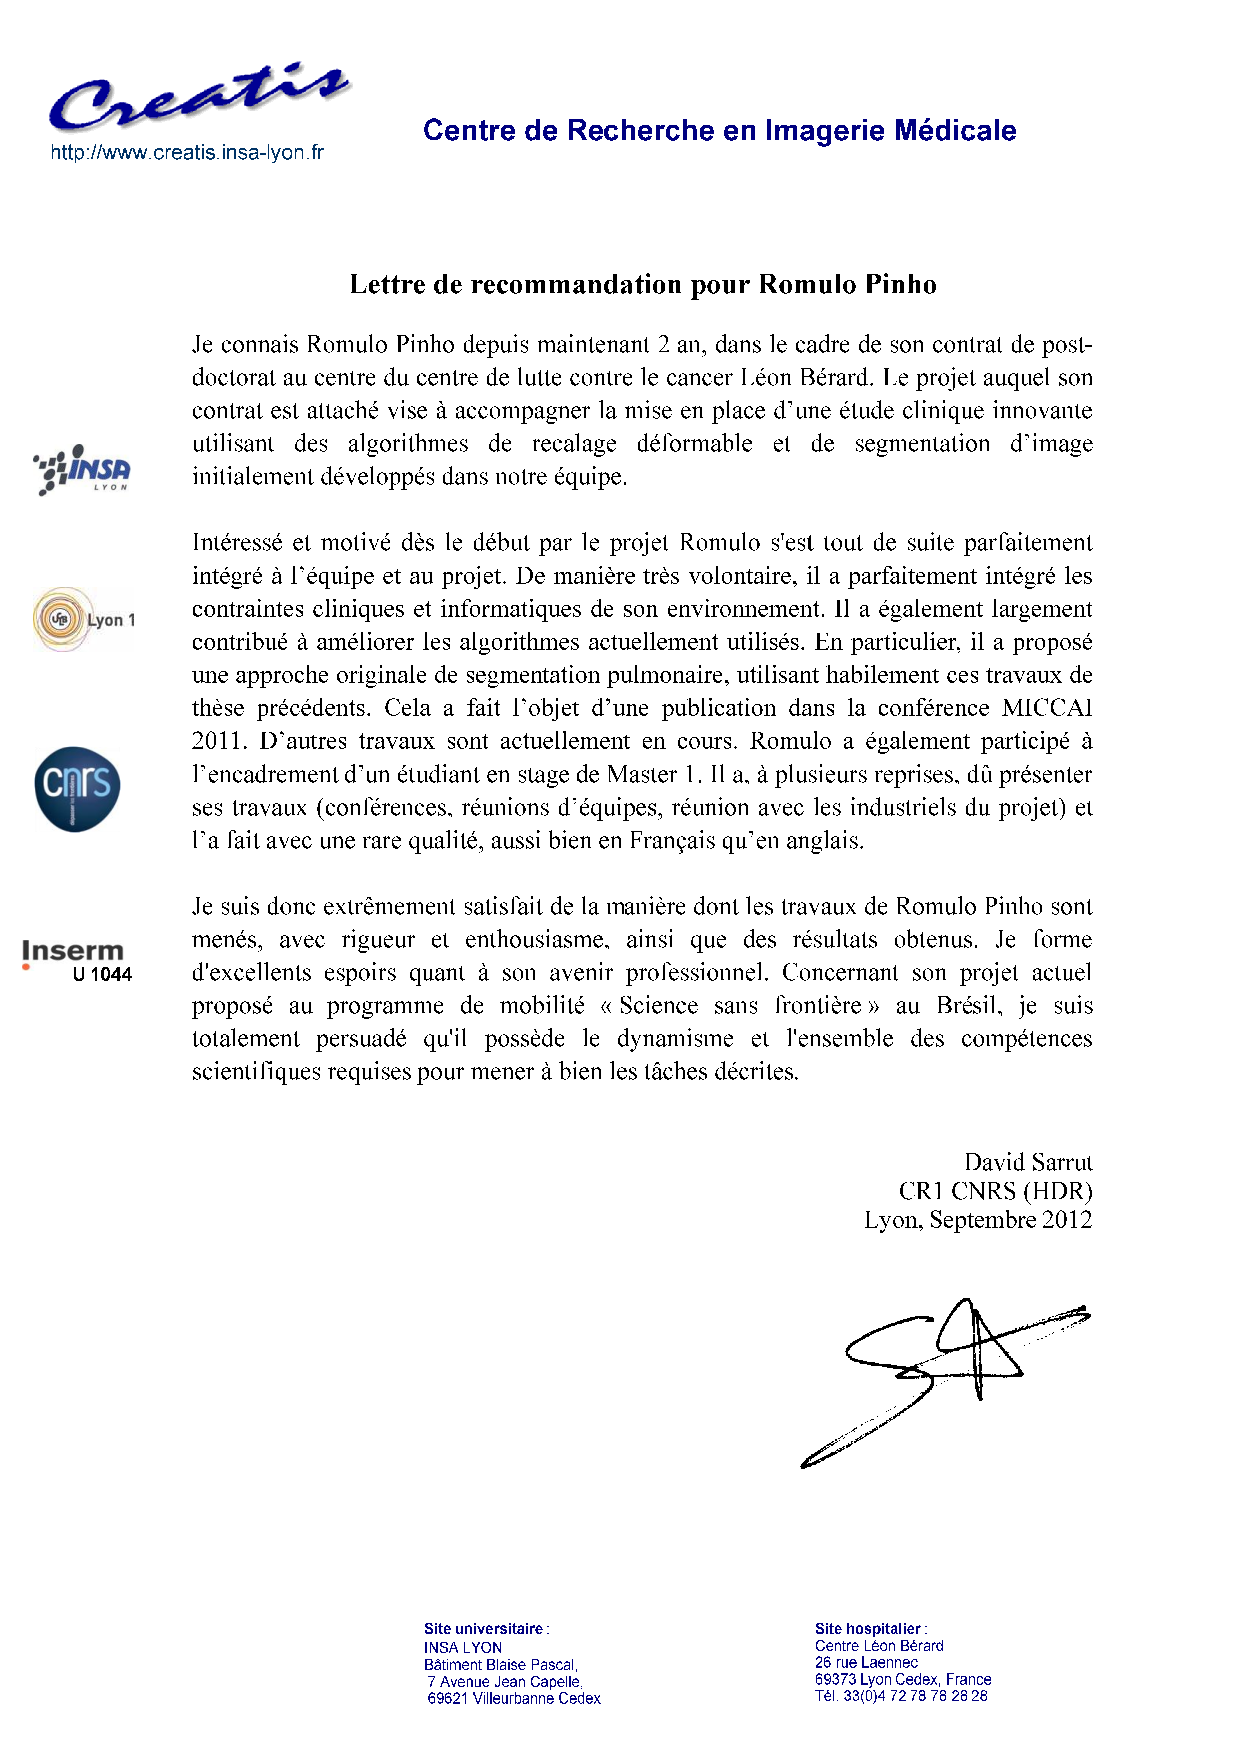
\includepdf[pages={1}]{david.pdf}
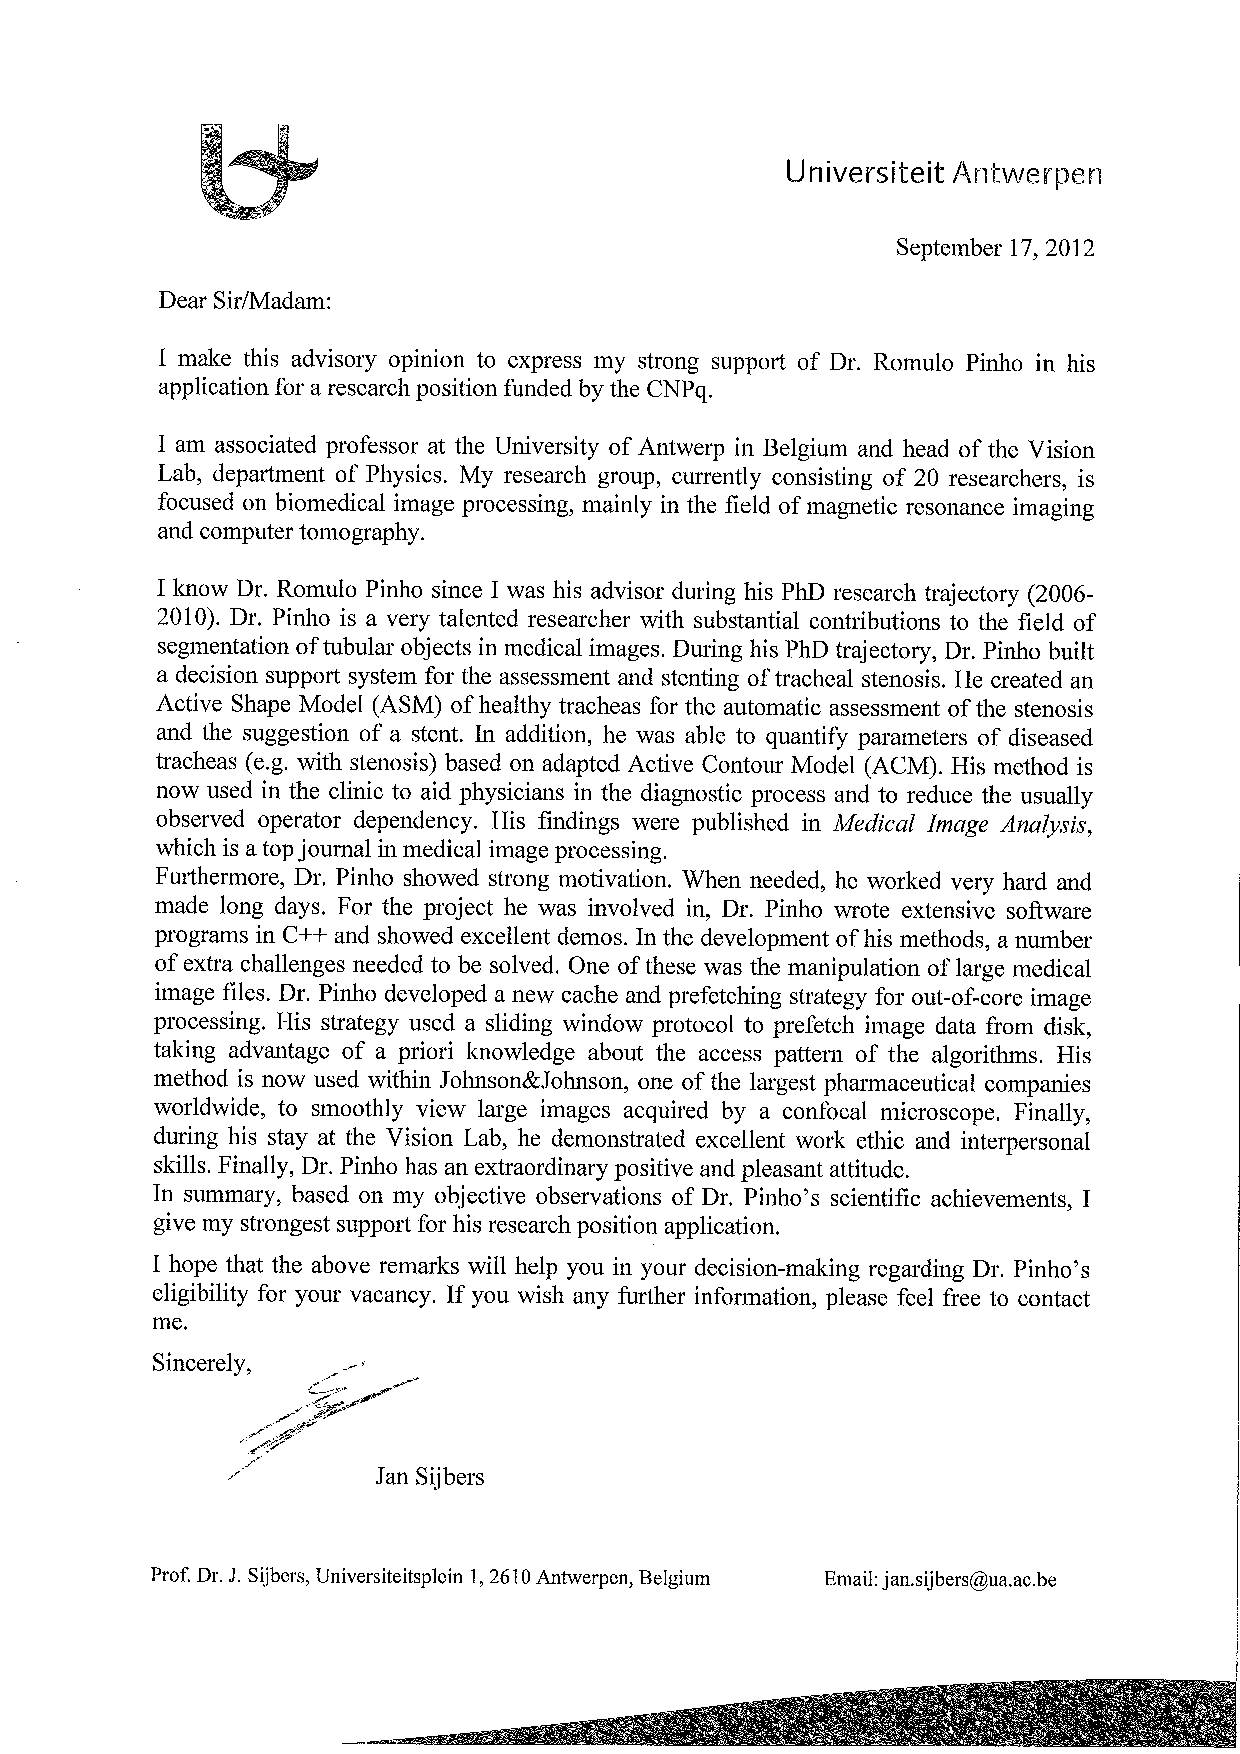
\includepdf[pages={1}]{jan.pdf}
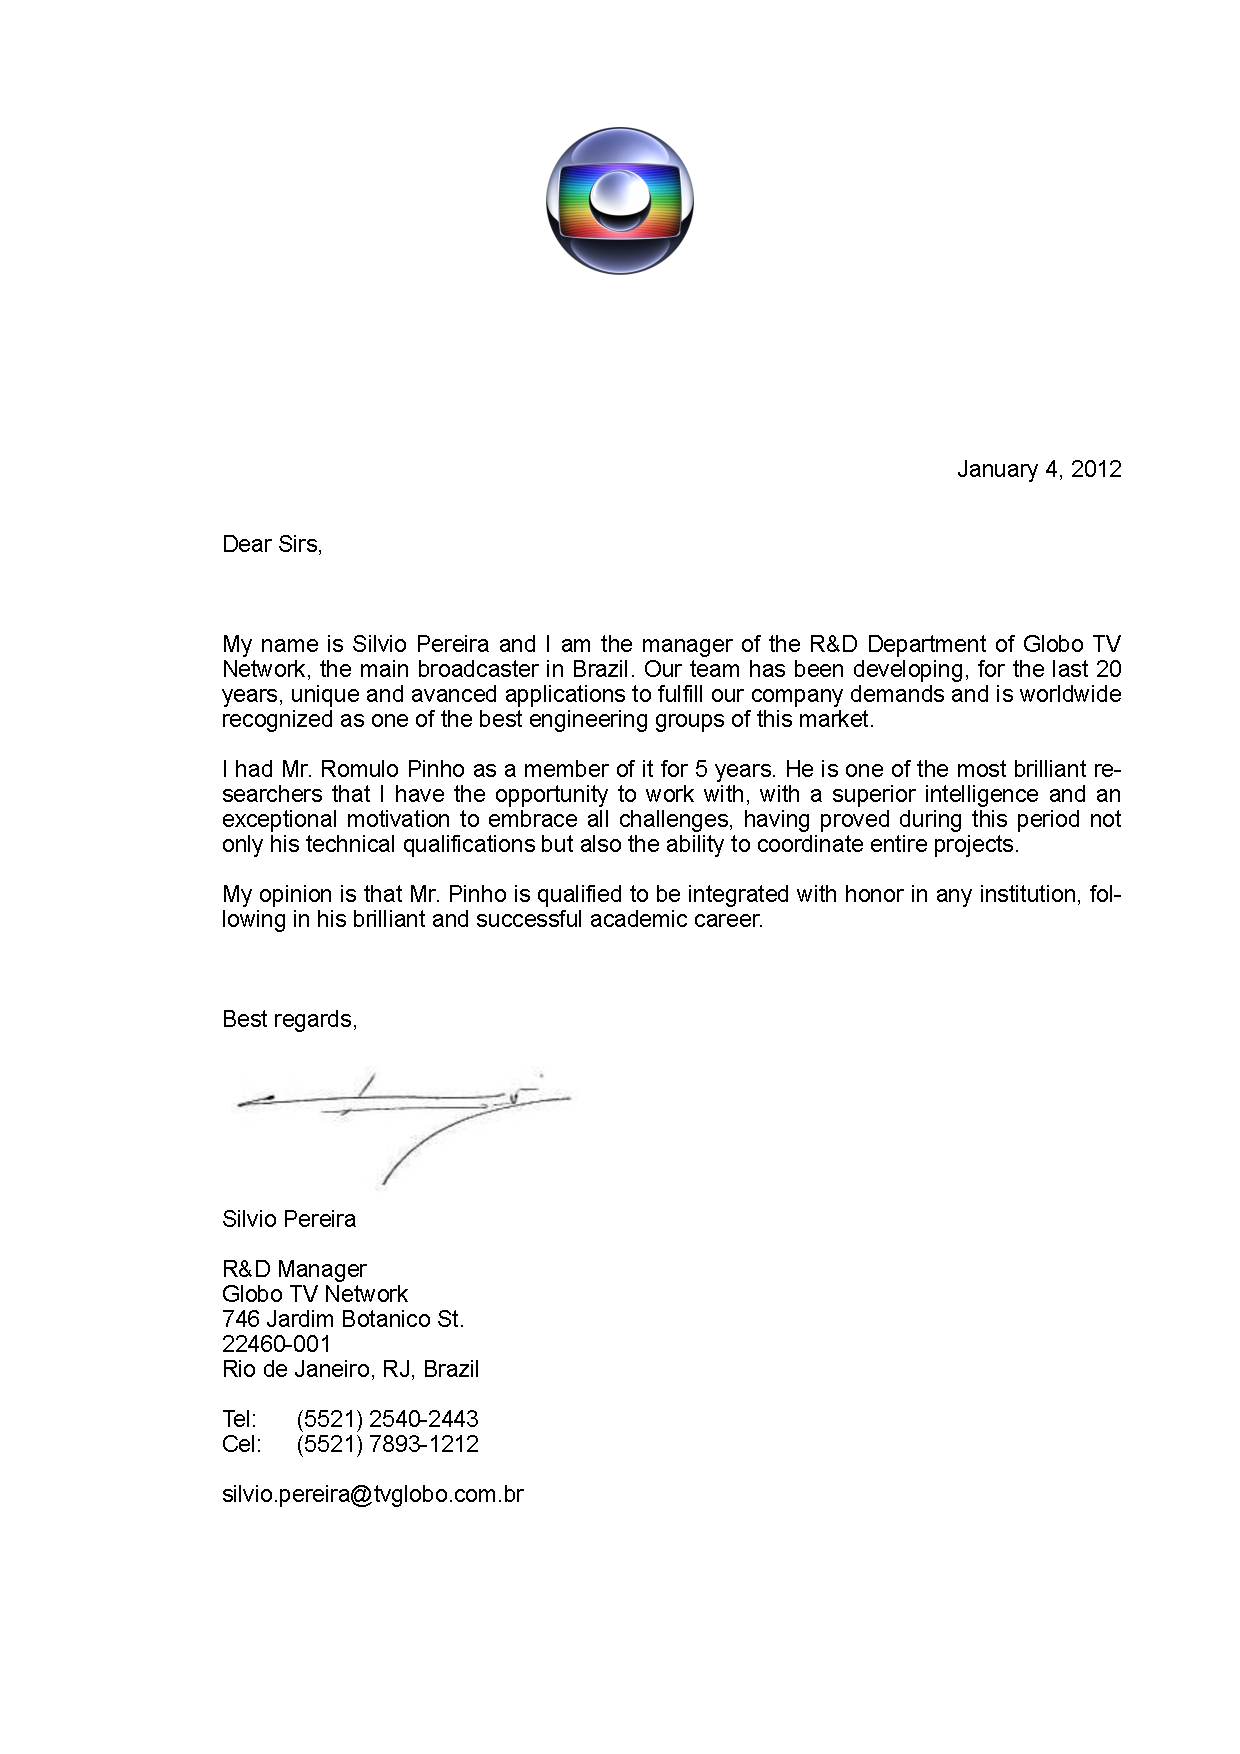
\includepdf[pages={1}]{silvio.pdf}
% \includepdf[pages={1}]{joao.pdf}



%\section{Conclusions}


\end{document}
